\chapter{Macrosegregation with solidification shrinkage}
%\chaptermark{Nonlinear Temperature Solver}
\begin{nolinkcolors} 
\minitoc
\end{nolinkcolors}
\newpage

% ======================
\section{Solidification shrinkage}
% ======================

Solidification shrinkage is, by definition, the effect of relative density change between the liquid and solid phases.
In general, it results in a progressive volume change during solidification, until the phase change has finished. 
The four stages in \cref{fig:real_ingot_stage_a,fig:real_ingot_stage_c,fig:real_ingot_stage_b,fig:real_ingot_stage_d} depict the volume change with 
respect to solidification time.
First, at the level of the first solid crust, near the local solidus temperature, the solid forms with a density greater than 
the liquid's. The subsequent volume decrease creates voids with a negative pressure, forcing the fluid to be sucked in the direction of the volume change 
(cf. \cref{fig:real_ingot_stage_b}). As a direct result of the inward feeding flow, the ingot surface
tends to gradually deform in the feeding direction, forming the so-called \emph{shrinkage pipe}, shown in \cref{fig:shrinkage_exp}. 
Since the mass of the alloy and its chemical species is conserved, 
a density difference between the phases ($\rhol < \rhos \implies \frac{\rhol}{\rhos}<1$) eventually leads 
to a different overall volume ($V^s<V^l$) once solidification is complete, as confirm the following equations:
%------------
\begin{subequations}
\begin{align}
& \rhol V^l = \rhos V^s  \\ 
& V^s = \frac{\rhol}{\rhos} V^l
\end{align}
\end{subequations}
%------------
Solidification shrinkage is not the only factor responsible for volume decrease. Thermal shrinkage in both solid and liquid phases, as well 
as solutal shrinkage in the liquid phase are also common causes in a casting process. 
However, thermal shrinkage is very important to apprehend, as temperature decreases in steel casting, usually exceeding a \SI{1000}{\udegC}, thus causing substantial density variations. 
%Henceforth, we will focus on shrinkage due to phase change.
%
%Talk and explain models in the literature that predict shrinkage (without or with macrosegregation): Beckermann, Wu ? \\
%Show and comment the experiments that have been done: Hebditch and Hunt, Smacs Hachani  ...
%
%\comment{ \textbf{Sutaria2012} talk about feeding paths, but more importantly they computed thermal shrinkage WITHOUT solving
%NavierStokes equations. To predict the interface shape, they solve a LS transport with an imposed velocity given by Gada et Sharma 2009}
%
%
%----------------
%
\begin{figure}[htbp]
\centering
%\begin{minipage}{.5\textwidth}
  \begin{subfigure}{0.3\textwidth}
    \centering
    \def\svgwidth{100pt}
	\import{Chapter4/Graphics/new/}{ingot_air_liq.pdf_tex}
	\caption{Initial state}
    \label{fig:real_ingot_stage_a}
  \end{subfigure}
  %\hfill
  \begin{subfigure}{0.3\textwidth}
    \centering
    \def\svgwidth{100pt}
	\import{Chapter4/Graphics/new/}{ingot_air_liq_mush_sol.pdf_tex} 
	\caption{Early intermediate state}
    \label{fig:real_ingot_stage_b}
  \end{subfigure}
%
\vskip\baselineskip
%======
%
  \begin{subfigure}{0.3\textwidth}
    \centering
    \def\svgwidth{100pt}
	\import{Chapter4/Graphics/new/}{ingot_air_mush_sol.pdf_tex}
	\caption{Late intermediate state}
    \label{fig:real_ingot_stage_c}
  \end{subfigure}
  %\hfill
  \begin{subfigure}{0.3\textwidth}
    \centering
    \def\svgwidth{100pt}
	\import{Chapter4/Graphics/new/}{ingot_air_sol.pdf_tex}
	\caption{Final state}
    \label{fig:real_ingot_stage_d}
  \end{subfigure}
  %
\caption{Schematic of the main cooling stages of an ingot against side and bottom mould walls (not shown)}
\label{fig:real_ingot_stages}
\end{figure}
%
%---------------------
%
%----------------------
\begin{figureth}
% textwidth 
{0.45}
%path 
{Chapter4/Graphics/shrinkage_exp.png}
% caption
{Sulphur prints of three ingots showing pipe formation at the top as a result 
of solidification shrinkage with various ingot inclination during casting \citep{onodera_effect_1959}.
Positive macrosegregation is clearly seen in this area, while A-shape and V-shape positive mesosegregates are detected
at the ingot's tips and center respectively.}
% label
\label{fig:shrinkage_exp}
\end{figureth}
%-----------------------------------
%
%
%============================================
\section{Choice of interface tracking}
%============================================
In chapter 2, several methods of interface tracking/capturing methods were presented 
along with their similarities and differences. In the case of solidification shrinkage,
the metal-air interface can be tracked with any method from the previously mentioned.
However, several reasons motivate us to settle on the level set method. 
First, the easiest solution is testing a method which already exists in \cimlib library.
The level set method was implemented by HERE as a framework for monolithic resolution. Since this work,
the method has been extensively used and improved in several projects mainly for multiphase flows, which is the 
main competence of the Computational Fluids LXXXX group at CEMEF. Another motivation is the compatibility
between \cimlib and \thercast, where the latter is the final destination of the code developed during for the Ph.D. thesis.
In its recent versions, \thercast handles laminar and turbulent ingot filling where the level set method is used 
to capture the free surface of the molten metal. Aside from the practical motivations, some technical aspects of the level
set method make it very attractive to apply it macroscopic surface tracking (in contrast to microscopic interface tracking, 
for instance the solid-liquid interface), such as topological properties that are readily available (e.g. curvature)
and accurate position compared to volume-based methods like VOF.
%
%============================================
\section{Multidomain formalism}
%============================================
In the previous chapters, we considered in our simulations the metal as a 
saturated mixture of solid and liquid during solidification.
It means that no gas phase may appear during the process, and this  this chapter.
The reason is we chose to describe our model in Eulerian description, 
for which we have considered a fixed grid to discretise the averaged conservation 
equations governing the phase change between the liquid and solid phases.
Furthermore, with the introduction of shrinkage, an increase in global density means 
that a gas phase should enter the domain to replace the shrunk volume.
At this point, several interfaces may be distinguished: liquid-solid ($l$-$s$), liquid-air ($l$-$a$) and solid-air ($s$-$a$), where 
we defined 2 phases ($l$ and $s$) belonging to the "Metal" domain denoted $M$, while the "Air" domain, denoted $A$, 
is made up of a unique phase, ($a$), with the same name. As a standard for this formalism, we consider that uppercase letters
are used for domains, while lowercase letters are used for phases.

The main idea behind the multidomain formalism, is to go from the classic 
conservations equations introduced by  volume averaging in chapter 2,
in the context of a solidifying two-phase system to generalise it by taking
into account a third gas phase, such as:
%-------------
\begin{align}
\label{eq:}
V^l + V^s + V^a = \rev \\
\gl + \gs + \ga = 1
\end{align} 
%-------------
while keeping a physical integrity with the former monodomain model. 
Then, one is free to choose a suitable numerical method to track the 
interfaces between the several phases. In our applications, we are particularly 
interested in keeping an indirect representation of the $l$-$s$ interface (dotted line in \cref{fig:rev_triphase})
using the volume averaging theory, while employing a different
method to track the $l$-$a$ and $s$-$a$ interfaces (dashed lines in \cref{fig:rev_triphase}) with the level set method. 
This allows switching to the latter method in a physically representative manner.

In this context, each domain can be seen as a material having a physical
interface with the other domains. As a consequence of our interpretation, 
the gas phase should not exist in the metal, which may naturally
occur if the thermodynamic conditions are in favour of nucleating and growing 
a new phase, or in the case of a gas that was trapped inside mould grooves.
%----------------------
\begin{figureth}
% textwidth 
{0.45}
%path 
{Chapter4/Graphics/REV_triphase.pdf}
% caption
{Schematic of a representative volume element containing 3 phases with distinct velocities, separated by 3 interfaces.
The dotted line is the indirectly tracked solid-liquid interface while the other dashed lines, air-liquid and air-solid
interfaces, are directly tracked.}
% label
\label{fig:rev_triphase}
\end{figureth}
%-----------------------------------
%
%
%------------
\subsection{Assumptions}
%------------
Each phase in the system has its own velocity, $\vl$, $\vs$ and $\va$, while the respective
interfaces $\liqsol$, $\liqair$ and $\solair$ have different and independent velocities, 
represented by $\vliqsol$, $\vliqair$ and $\vsolair$. Note that the solid-liquid interface
velocity was denoted $\vstar$ in the previous chapters as no more than two phases were considered.
The first major assumption is that the solid phase, once formed from the liquid, is fixed and rigid.
It means that no subsequent deformation may occur and therefore $\vsolair$ reduces to vector zero.
Moreover, we use the already introduced volume averaging principles to write locally for any quantity $\psi$:
%------------
\begin{subequations}
\begin{align}
\label{eq:}
\avg{\psi} &= \avg{\psi^l} + \avg{\psi^s} + \avg{\psi^a} \\
			&= \gl \psi^l + \gs \psi^s  + \ga \psi^a
\end{align}
\end{subequations}
%------------
where volume fractions, $\gphi$, for each phase $\phi$ were used. \citet{rappaz_numerical_2003} define
the volume fraction by writing a general expression inside the representative volume $\rev$:
%------------
%\begin{subequations}
\begin{align}
\label{eq:}
\gphi = \frac{1}{\rev} \integral{\rev}{\chi^\phi(x,t)}{\Ohm} = \avg{\chi^\phi}
\end{align}
%\end{subequations}
%------------
where the integrated quantity is an indicator (or presence) function relative to phase $\phi$, which
defines the volume of this phase in the system, $\Ohm^\phi$, as follows:
%------------
%\begin{subequations}
\begin{align}
\label{eq:}
\chi^\phi(x,t)=
\begin{cases}
  1 	& \text{ if } x \in \Ohm^\phi \\ 
  0 	& \text{otherwise}
\end{cases}
\end{align}
%\end{subequations}
%------------
Any phenomenon that may displace an interface, whether by phase change or a phase motion, is 
mathematically translated by variations of the presence function, such that its total derivative for each phase
satisfies the following:
%
%------------
\begin{align}
\label{eq:transport_presence}
& \frac{d \chi^\phi}{dt} = \tempup{\chi^\phi} + \vstar \cdot \nabvec \chi^\phi = 0
\end{align}
%------------
%
If we consider the liquid phase, the variations of any quantity, named $\psi$, are given by:
%------------
\begin{align}
\label{eq:}
& \avg{{\tempup{\psi^l}}} = \tempup{\avg{\psi^l}}
							- \frac{1}{\rev} \integral{l-a}{\psi^l \vliqair \cdot \nliqair}{\Gamma}
							- \frac{1}{\rev} \integral{l-s}{\psi^l \vliqsol \cdot \nliqsol}{\Gamma} \\
& \avg{\nabvec \psi^l} =  \nabvec{\avg{\psi^l}} 
							+ \frac{1}{\rev} \integral{l-a}{\psi^l \nliqair}{\Gamma} 
							+\frac{1}{\rev} \integral{l-s}{\psi^l \nliqsol }{\Gamma} \\
& \avg{\nabvec \cdot \vec{\psi}^l} =  \nabvec \cdot {\avg{\vec{\psi}^l}} 
							+ \frac{1}{\rev} \integral{l-a}{\vec{\psi^l} \cdot \nliqair }{\Gamma} 
							+\frac{1}{\rev} \integral{l-s}{\vec{\psi^l} \cdot  \nliqsol }{\Gamma}							
\end{align}
%------------
\Cref{eq:transport_presence} can be recast with the level set method by using the smoothed Heaviside function in the metal.
For the metal, this function is equal to one and decreases to zero in the air in a smooth way across both interfaces, solid-air and liquid-air.
Since the solid phase is assumed fixed without possible deformation, and knowing that air is assumed incompressible, 
the solid-air interface does not move, leading to the following equation: 
%------------
\begin{align}
\label{eq:transport_heaviside}
& \frac{d \heavisideM}{dt} = \tempup{\heavisideM} + \vliqair \cdot \nabvec \heavisideM = 0
\end{align}
%------------
%======================
\section{FE partitioned model}
%--------------------------------------------------
%
In this section, we start from a the monodomain finite element model presented in \cref{sec:monodomain} that was relevant to the metal only, 
referred to by the superscript $M$, then present the essential assumptions and formulations 
that allow predicting solidification shrinkage in a Eulerian context that introduces
another domain, the air, referred to by the superscript $A$.
\subsection{In the metal}
%
\subsubsection{Mass and momentum conservation}
By assuming a fixed solid phase ($\vs=\vec{0}$), the average velocity in the metal reduces only to liquid's average velocity.
Therefore, we can write:
%------------
\begin{align}
\label{eq:vitmetal}
& \vM = \vit = \gl \vl 
\end{align}
%------------
With \cref{eq:vitmetal}, the mass balance in the metal writes:
%------------
\begin{subequations}
\begin{align}
& \tempup{\avg{\rho}^M} + \nabla \cdot \avg{\rho \vec{v}}^M  = 0 \\ 
& \tempup{\avg{\rho}^M} + \nabla \cdot \brac{ \gl \rhol \vl} = 0 \\ 
& \tempup{\avg{\rho}^M} + \rhol \nabla \cdot \brac{ \gl \vl} 
	+ \gl \vl \cdot  \nabvec \rhol = 0 \\	
\label{eq:mass_balance_metal}
& \nabla \cdot \vit 
= -\frac{1}{\rhol} \brac{\tempup{\avg{\rho}^M }+ \vit \cdot  \nabvec \rhol}
\end{align}
\end{subequations}
%------------
\Cref{eq:mass_balance_metal} explains the flow due to shrinkage. A negative divergence term means that a liquid feeding 
is necessary to compensate for the density difference, hence acting as a flow driving force in the melt.
Additional terms should appear in the other conservation equations, balancing the volume 
change in the heat and species transport.
%
%-----------------------------------
%\subsection{Momentum Conservation}
%-----------------------------

When the metal's density was considered constant during solidification, 
the assumption of an incompressible system made it possible to
use the Boussinesq approximation. However, in the case of solidification shrinkage, 
the average density ${\avg{\rho}}^M$
varies, as it depends on the solidification path as well as on $\rhos$ and $\rhol$ which are not equal nor constant.
Therefore, the incompressibility condition may not be applicable. In such case, 
the earlier given system \cref{eq:Navier-Stokes2} is reformulated without 
any reference value for density:
%------
\begin{equation}
\label{eq:momentum_balance_metal}
   \left\{
   \begin{aligned}
      & \rhol \brac{\tempup{ \vit } + \frac{1}{\gl} \nabvec \cdot \brac{\vit \times \vit}} = \\
	  &- \gl\nabvec \pl - 2 \mul \nabvec \cdot \brac{\nabmat \vit + \nabmattransp \vit}
	  - \gl \mul \K^{-1} \vit + \gl \rhol \gravity\\ \\
      & \nabla \cdot \vit = -\frac{1}{\rhol} \brac{\tempup{\avg{\rho}^M} + \vit \cdot  \nabvec \rhol}
    \end{aligned}
    \right.
\end{equation}
%------------
%====================================================================
\subsubsection{Energy conservation}
% ======================
In the energy equation, a volumetric source term accounts for the heat dissipation 
caused by the shrinking metal volume. Before writing the new equation, we make the following assumptions:
% ======================
%Assumptions
% ======================
\begin{itemize}
\itemsep0em
%\item The thermal conductivity is constant for both phases: $\avg{\kappa} = \ks = \kl= \kappa $ 
%\item consideration of a fixed solid ($ \vec{v}^s=\vec{0} $).
\item consequence of the static solid phase: $\avg{\rho h \vec{v}} = \gl \rhol \hl \vl +  \cancel{\gs \rhos \hs \vs} = \gl \rhol \hl \vl$ 
%\item The system's enthalpy may thermodynamically evolve with pressure, knowing that $h=e+\frac{p}{\rho}$, where $e$ is the internal energy and $p$ is the pressure. It infers that the heat transport equation may contain a contribution attributed to volume compression/expansion:
%\begin{align}
%			 \frac{\partial p}{\partial t}+\nabla \cdot \brac{p \vec{v}}
%			 = \frac{\partial p}{\partial t}+ p \nabla \cdot \vec{v} + \vec{v} \cdot \nabvec p 
%\end{align}
%In the literature, this contribution has been always neglected, even when accounting for solidification
%shrinkage, owing to the small variations of pressure.
\item the heat generated by mechanical deformation, $\mathbb{S}:\dot{\varepsilon}$, is neglected
%\begin{enumerate}
%\item $\avg{\rho h}= \gl \rhol \hl + \gs \rhos \hs $
%\end{enumerate}
\end{itemize}
% ======================
%Formulation
% ======================
The unknowns in the energy conservation are the average volumetric enthalpy $\avg{\rho h}^M$ and temperature $T$.
The energy conservation equation writes:
\begin{subequations}
\begin{align}
	& \tempup{\avg{\rho h}^M} + \nabla \cdot \avg{\rho h \vec{v}}^M 
	= \nabla  \cdot \brac{\avg{\kappa}^M \nabvec T } \\
	& \tempup{\avg{\rho h}^M} + \nabla \cdot \brac{ \gl \rhol \hl \vl} 
	= \nabla  \cdot \brac{\avg{\kappa}^M \nabvec T } \\
	& \tempup{\avg{\rho h}^M}
		+ \vit \cdot \nabvec \brac{\rhol \hl}
		= \nabla  \cdot \brac{\avg{\kappa}^M \nabvec T }
		  - \rhol \hl  \nabla \cdot \vit \\   
	\label{eq:energy_balance_metal}
	& \tempup{\avg{\rho h}^M}
		+ \vit \cdot \nabvec \brac{\rhol \hl}
		= \nabla  \cdot \brac{\avg{\kappa}^M \nabvec T }
		+ \hl \brac{\tempup{\avg{\rho}^M} + \vit \cdot  \nabvec \rhol} 
\end{align}
\end{subequations}
%\begin{align}
% \boxed{ \frac{\partial \avg{\rho h}}{\partial t} 
%		+ \rhol \vit \cdot \nabvec \hl
%		= \nabla  \cdot \brac{\kappa \nabvec T }
%		+ \brac{\rhos-\rhol} \hl \frac{\partial  \gs}{\partial t}}
%\end{align}
%----------------
%
%In order to keep things simple, the term "enthalpy" will refer henceforth to "volume enthalpy",
%otherwise, we will explicitly use the term "mass enthalpy". It is important to understand the 
%meaning of the terms in equation \cref{eq:energy_balance}.
%The first term in the left-hand side is the temporal change in the system's average enthalpy,
%i.e. a temporal change in the volume enthalpy of any of the phases in the course of solidification.
%The second LHS term is a dot product between the superficial liquid velocity and the the gradient
%of the liquid's enthalpy. Since phase densities are constant in our case, the gradient term reduces
%to the liquid's mass enthalpy. If we consider a representative volume element (RVE) in the liquid
%phase, far from the mushy zone, we can stipulate:
%
%--------------
%\begin{align}
%\label{eq:gradient_liquid_enthalpy}
%& \nabvec \hl = C_p^l \nabvec T
%\end{align}
%--------------
%
%assuming that the phase mass specific heat, $ C_p^l $, is constant. Therefore, the liquid enthalpy
%is advected in the case where the velocity vector is not orthogonal to the temperatre gradient.
%The advection reaches its maximum when the two vectors have the same direction. Consider, for instance,
%a filled ingot with a cooling flux applied to its bottom surface. If the density variation with temperature
%were to be neglected, then the sole mechanical driving force in the melt is the density jump at the solid-liquid
%interface ahead of the mushy zone. The temperature gradient in such a case is vertical upward, while the velocity
%vector is in the opposite direction. The advective term writes:
%
%--------------
%\begin{align}
%\label{eq:enthalpy_advection}
%& \rhol \vit \cdot \nabvec \hl = - \rhol C_p^l \norm{\vit} \norm{\nabvec T}
%\end{align}
%--------------
%
%----------------------------
%\begin{figure}
%\centering
%\begin{subfigure}[h!]{0.3\textwidth}\centering % h! or H
%	\def\svgwidth{100pt}
%	\import{Chapter4/Graphics/}{Ingot_sl_1D_a.pdf_tex}
%	\caption{Initial state}
%	\label{fig:ingot_1d_a}
%\end{subfigure}
%\begin{subfigure}[h!]{0.3\textwidth}\centering % h! or H
%	\centering
%	\def\svgwidth{100pt}
%	\import{Chapter4/Graphics/}{Ingot_sl_1D_c.pdf_tex}
%	\caption{Solidification onset}
%	\label{fig:ingot_1d_c}
%\end{subfigure}
%\begin{subfigure}[h!]{0.3\textwidth}\centering % h! or H
%	\centering
%	\def\svgwidth{100pt}
%	\import{Chapter4/Graphics/}{Ingot_sl_1D_d.pdf_tex}
%	\caption{Final state}
%	\label{fig:ingot_1d_d}
%\end{subfigure}
%\caption{Effect of one-dimensional shrinkage flow on a solidifying ingot}
%\end{figure}
%----------------------
%
%We see that the second LHS term in equation \eqref{eq:energy_balance} acts as 
%a heat source at the interface between the the phases, in this particular solidification
%scenario. 
The second term in the RHS of \cref{eq:energy_balance_metal} is a heat power (of unit $Wm^{-3}$) that adds 
to the system in the mushy zone. This term is proportional to the solidification rate and expresses 
the heat generated in regions where the average density is changing and/or a gradient of liquid density is being advected.
% ======================
\subsubsection{Species conservation}
% ======================
The last conservation principle is applied to the chemical species or solutes. This principle allows predicting
macrosegregation when applied to a solidification system, along with the mass, momentum and energy balances.
However, the conservation equation should be reformulated in the case of a melt flow driven by shrinkage.
% ======================
Assumptions
% ======================
\begin{itemize}
\itemsep0em
%\item the alloy is binary, i.e. it is composed from one solute, and hence the notation of the average composition
%		without a solute index: $\wavg$ for the mass composition and $\avg{\rho w}$ for the volume composition
\item %the solid fraction is determined assuming complete mixing in both phases, hence the lever rule is applied. 
	  the solidification path is tabulated using thermodynamic data at equilibrium
\item the macroscopic solute diffusion coefficient $D^s$ in the solid phase is neglected in the mass diffusive flux term.
\item consequence of the static solid phase: $\avg{\rho w \vec{v}}^M = \gl \rhol \wl \vl +  \cancel{\gs \rhos \ws \vs} = \gl \rhol \wl \vl$ 
\end{itemize}
% ======================
%Formulation
% ======================
The species conservation is pretty similar the energy conservation formulated in the previous section. 
The main difference is the breakup of the volumetric variable $\avg{\rho w}^M$ into a product of density  $\avg{\rho}^M$ and the mass concentration $\avg{w}^M$.
For a binary alloy, we write:
%
%--------------------------
%
\begin{subequations}
\begin{align}
 & \tempup{\avg{\rho w}^M} + \nabla \cdot \avg{\rho w \vec{v}}^M - \nabla  \cdot \brac{\avg{\Dl} \nabvec \brac{\rhol \wl} } = 0 \\
 %
 & \avg{\rho}^M \tempup{\avg{w}^M} + \avg{w}^M \tempup{\avg{\rho}^M} 
	+ \nabla \cdot \brac{\gl \rhol \wl \vl} 
	- \nabla \cdot \brac{\gl \Dl \nabvec \brac{\rhol \wl} } = 0 \\
 %
 \label{eq:species_1}
  \begin{split}
	& \avg{\rho}^M \tempup{\avg{w}^M} + \avg{w}^M \tempup{\avg{\rho}^M} 
	+ \brac{\rhol \wl} \nabla \cdot \vit + \vit \cdot \nabvec \brac{\rhol \wl} \\
	& - \nabla \cdot \brac{\gl \Dl \nabvec \brac{\rhol \wl} } = 0 
  \end{split}
%
\end{align}
\end{subequations}
%--------------------------
The mass balance gives the following relation when the liquid density is constant:
%--------------------------
\begin{align}
\label{eq:species_divV}
\nabla \cdot \vit = -\frac{1}{\rhol} \brac{\tempup{\avg{\rho}}^M}
\end{align}
%----------------
If we use the result of \cref{eq:species_divV} in \cref{eq:species_1}, then we get the following equation:
\begin{align}
\avg{\rho}^M \tempup{\avg{w}^M}  + \avg{w}^M \tempup{\avg{\rho}^M} =
\wl \tempup{\avg{\rho}^M}  - \vit \cdot \nabvec \brac{\rhol \wl} + \nabla \cdot \brac{\gl \Dl \nabvec \brac{\rhol \wl} }
\end{align}
%
Applying Voller-Prakash \citep{voller_modelling_1989} variable splitting, the system ends up with only one variable, $\avg{w}^M$. 
The splitting is done as follows:
\begin{align}
\label{eq:voller_prakash}
\wl = \brac{\wl}^t + \avg{w}^M - \brac{\avg{w}^M}^t
\end{align}
%
where the superscript $t$ refers to the previous time step. The chemical species conservation writes:
%
\begin{subequations}
\begin{align}
  \begin{split}
	& \avg{\rho}^M \tempup{\avg{w}^M}  + \cancel{\avg{w}^M \tempup{\avg{\rho}^M}} = \\
	& \cancel{\avg{w}^M \tempup{\avg{\rho}^M}}  - \rhol \vit \cdot \nabvec \avg{w}^M + \nabla \cdot \brac{\gl \rhol \Dl \nabvec \avg{w}^M } \\
	& + \tempup{\avg{\rho}^M} \crochet{\brac{\wl}^t -  \brac{\avg{w}^M}^t} - \rhol \vit \cdot \nabvec \brac{\brac{\avg{w}^M}^t -\brac{\wl}^t} \\
	%& + \nabla \cdot \crochet{\gl \rhol \Dl  \nabvec \brac{ \brac{\wl}^t - \avg{w}^t } }
  \end{split} \\ 
    \begin{split}
	& \avg{\rho}^M \tempup{\avg{w}^M}  + \rhol \vit \cdot \nabvec \avg{w}^M - \nabla \cdot \brac{\gl \rhol \Dl \nabvec \avg{w}^M}=\\
	& - \tempup{\avg{\rho}^M} \crochet{\brac{\avg{w}^M}^t - \brac{\wl}^t} + \rhol \vit \cdot \nabvec \brac{\brac{\avg{w}^M}^t -\brac{\wl}^t} \\
	& - \nabla \cdot \crochet{\gl \rhol \Dl  \nabvec \brac{\brac{\avg{w}^M}^t -\brac{\wl}^t} }
  \end{split}
\end{align}
\end{subequations}
%
%\begin{subequations}
%\begin{align}
%	& \frac{\partial \avg{\rho w}}{\partial t} 
%		+ \rhol \wl  \nabla \cdot \vit
%		+ \vit \cdot \nabvec \brac{\rhol \wl}
%		= \nabla  \cdot \brac{\gl \rhol D^l \nabvec \wl } \\   
%	& \frac{\partial \avg{\rho w}}{\partial t} 
%		+ \cancel{\rhol} \wl  \frac{\rhol-\rhos}{\cancel{\rhol}} \frac{\partial  \gs }{\partial t}
%		+ \vit \cdot \nabvec \brac{\rhol \wl}
%		= \nabla  \cdot \brac{\gl \rhol D^l \nabvec \wl } \\ 
%	& \frac{\partial \avg{\rho w}}{\partial t} 
%		+ \brac{\rhol-\rhos} \wl \frac{\partial  \gs }{\partial t}
%		+ \vit \cdot \nabvec \brac{\rhol \wl}
%		= \nabla  \cdot \brac{\gl \rhol D^l \nabvec \wl }        
%\end{align}
%\end{subequations}
%------------------------------
\begin{align}
\label{eq:solute_balance_metal}
\begin{split}
 & \avg{\rho} \tempup{\avg{w}^M}  + \rhol  \vit \cdot \nabvec \avg{w}^M - \nabla \cdot \brac{\gl \rhol \Dl \nabvec \avg{w}^M}=\\
 &	 - \tempup{\avg{\rho}^M} \crochet{\brac{\avg{w}^M}^t - \brac{\wl}^t} \\ 
 &	 + \rhol \vit \cdot \nabvec \brac{\brac{\avg{w}^M}^t -\brac{\wl}^t}
 	 - \nabla \cdot \crochet{\gl \rhol \Dl  \nabvec \brac{\brac{\avg{w}^M}^t -\brac{\wl}^t} }
  \end{split}
  \end{align}
%--------------
It is noted that \cref{eq:solute_balance_metal} is valid only if both densities $\rhol$ and $\rhos$
are constant but have different values. Since density changes are incorporated in this equation, 
inverse segregation following solidification shrinkage is predicted.
For the case where macrosegregation is solely due to fluid flow generated by natural or forced convection, 
i.e. no shrinkage occurs whether due to thermal-solutal contraction or phase change, 
the overall volume remains constant, hence density is constant. 
In this situation, $\rhos=\rhol=\avg{\rho}$ and the term $\partial \avg{\rho}/\partial t$ therefore vanishes.
After dividing both sides by $\avg{\rho}=\rhol$, \cref{eq:solute_balance_metal} reduces to:
%------------------------------
\begin{align}
\label{eq:solute_balance_metal_incompressible}
 \begin{split}
      & \tempup{\avg{w}^M}  + \vit \cdot \nabvec \avg{w}^M - \nabla \cdot \brac{\gl \Dl \nabvec \avg{w}^M} \\
	  & = \vit \cdot \nabvec \brac{\brac{\avg{w}^M}^t -\brac{\wl}^t}
	 - \nabla \cdot \crochet{\gl \Dl \nabvec \brac{\brac{\avg{w}^M}^t -\brac{\wl}^t} } 
  \end{split}
\end{align}
%--------------
%
%====================================================================
\subsection{In the air}
The presence of an air domain in our approach is important to follow the free surface of the solidifying metal.
For this particular reason, some assumptions are introduced and explained in this section in order to limit unnecessary treatment within
the air, since it does not undergo phase change. It should be reminded that we consider air as a single-phase system, hence superscripts $A$ and $a$
are interchangeably used. 
%
\subsubsection{Mass and momentum conservation}
%-----------------
To simplify fluid flow resolution in the air, we consider it as incompressible. This assumption is acceptable in the context
of casting processes where air velocity has an insignificant order of magnitude. Therefore, the free metal surface is not 
disturbed by air flow in its vicinity. With the incompressibility of air, we are saying that any deformation of the free surface 
is solely due to an air mass increase, coming from the system boundaries. The mass balance hence writes:
%------------
\begin{align}
\label{eq:mass_balance_air}
& \nabla \cdot \vA = \nabla \cdot \va = 0
\end{align}
%------------
The air flow is governed by time-dependent incompressible Navier-Stokes equations, as previously done for the metal:
%------
\begin{equation}
\label{eq:momentum_balance_air}
   \left\{
   \begin{aligned}
      & \rhoa \brac{\tempup{ \va } + \nabvec \cdot \brac{\va \times \va}} = \\
	  &- \nabvec \pa - 2 \mua \nabvec \cdot \brac{\nabmat \va + \nabmattransp \va}
	   + \rhoa \gravity\\ \\
      & \nabla \cdot \va = 0
    \end{aligned}
    \right.
\end{equation}
%------------
The air density $\rhoa$ is considered constant along the casting process, 
therefore thermal gradients in the air that arise due to the low
thermal conductivity, do not generate any flow, i.e. no Boussinesq approximation 
is made on the term $\rhoa \gravity$ in \cref{eq:momentum_balance_air}.
%-----------
\subsubsection{Energy conservation}
%-----------------
It was mentioned in the introduction of the current section that air is a single-phase system
that cannot undergo any phase change. Therefore, heat transfer in this domain simplifies to pure 
thermal conduction with a low thermal conductivity coefficient, $\ka$.
The energy balance governs the air enthalpy $\avg{\rho h}^A$ (which is equal to $\rhoa \ha$ 
in the current context) as follows:
\begin{subequations}
\begin{align}
	& \tempup{\avg{\rho h}^A} + \nabla \cdot \avg{\rho h \vec{v}}^A 
	= \nabla  \cdot \brac{\avg{\kappa}^A \nabvec T } \\
	& \tempup{\avg{\rho h}^A} + \nabla \cdot \brac{ \rhoa \ha \va} 
	= \nabla  \cdot \brac{\ka\nabvec T } \\
	\label{eq:energy_balance_air}
	& \tempup{\avg{\rho h}^A}
		+ \va \cdot \nabvec \brac{\rhoa \ha}
		= \nabla  \cdot \brac{\ka\nabvec T }
\end{align}
\end{subequations}
%------------
\subsubsection{Species conservation}
%-----------------
The composition of alloying elements is crucial quantity to predict in this work. Nevertheless, such prediction is only relevant
in the metallic alloy, even if the air is also made up of other chemical species (nitrogen, oxygen ...). For this obvious reason,
the species conservation equation should not be solved in the air, but that of course is contradictory to the principle of a monolithic approach.
Consequently, we should compute the conservation of chemical species in the air and the metal, but limit as much as possible
the influence of the former, in a way to prevent any solute transport between these domains. To do so, we consider that
both domains have the same solute content: $\avg{\Cnominal}^M=\avg{\Cnominal}^A$.
Moreover, the computed air velocity, $\va$, will not be used but rather a zero-velocity vector instead, thus suppressing the solute advection term.
As for solute diffusion, a very low macroscopic solute diffusion 
coefficient is used, ensuring that its order of magnitude is at most a thousand times less than that in the melt, $\Da \lll \Dl$.
The low artificial diffusion in the air may slightly violate the wanted no-exchange condition at the air-liquid interface, 
but it is acceptable since suppressing the diffusion term in the air would result in a numerically stiff partial differential equation.
%--------------
\begin{align}
  \label{eq:solute_balance_air}
	& \avg{\rho}^A \tempup{\avg{w}^A}
	%+ \va \cdot \nabvec \brac{\rhoa \wa}
	- \nabla \cdot \brac{\Da \nabvec \brac{\rhoa \wa} } = 0
\end{align}
%--------------
%
In contrast to \cref{eq:solute_balance_metal} for the metal, solute balance in the air, given by \cref{eq:solute_balance_air}, provides
a linear equation as we consider a special case where the domain is monophase, therefore:  $\avg{w}^A = \avg{w}^a$ for all $(x,t)$.
Otherwise, we would have applied the variable decomposition done earlier in \cref{eq:voller_prakash} to linearise the equation.
%
\section{FE monolithic model}
%---------------------------------------
The monolithic model combines all conservation equations derived for metal and air in a unique set of equations, to be solved on a fixed mesh. 
This can be accomplished by using the Heaviside function (defined in \cref{sec:heaviside}) relative to each domain, creating a mixture of properties that
vary across the interface according to a specified mixing law. However, one of the main technical difficulties of the monolithic resolution is that the
obtained equation should be consistent with each domain's original equation regarding its shape and terms, making its resolution easier. 
While for energy and solute balances the procedure is straightforward, for fluid mechanics it is not with the presence of the Darcy 
dissipative term in the metal's Navier-Stokes system.
%
%---------------------------------------
\subsection{Darcy term in the air}
%------
How to mix liquid fraction, best using harmonic or arithmetic, in order to replicate the effect the of non slip condition at top for example \\
Put the python plots from the presentations in "TEXUS monolithic" \\
Put video animations of PSEUDO SMACS 2D without and with LS ???
%------------------
\subsection{Interface treatment}
%
The level set method, like any other interface tracking/capturing method, needs defining a convenient way of coupling
the velocity field on the one hand, which is the solution provided by solving momentum conservation equations, with the 
interface position on the other hand. The question is "how does the velocity field transport the interface?". The answer
is potentially one of two possibilities: classical coupling or modified coupling. In the next subsections, we discuss
the technical details of each approach and the hurdles that come with it.
%---------
\subsubsection{Classical coupling}
%
A "classical" coupling comes in the sense of "unmodified" coupling. This approach consists of taking the output of the fluid mechanics
solver, then feed it as raw input to level set transport solver. The physical translation would be that the interface motion is dictated
by the fluids flow in its vicinity. No treatment whatsoever is done between the two mentioned steps. While conservation principles are best
satisfied with this approach, the latter yields some drawbacks, preventing its application in a generic way.
For instance, the free liquid surface is not necessarily horizontal at all times and that can lead to the wrong shrinkage profile
when solidification is complete.
\comment{present the example of unstable interface when the ratio between fluids properties became greater than some value+discussion} 
%----------------------------
\begin{figure}[htbp]
\centering
 \begin{subfigure}[t]{0.4\textwidth}
    \centering
	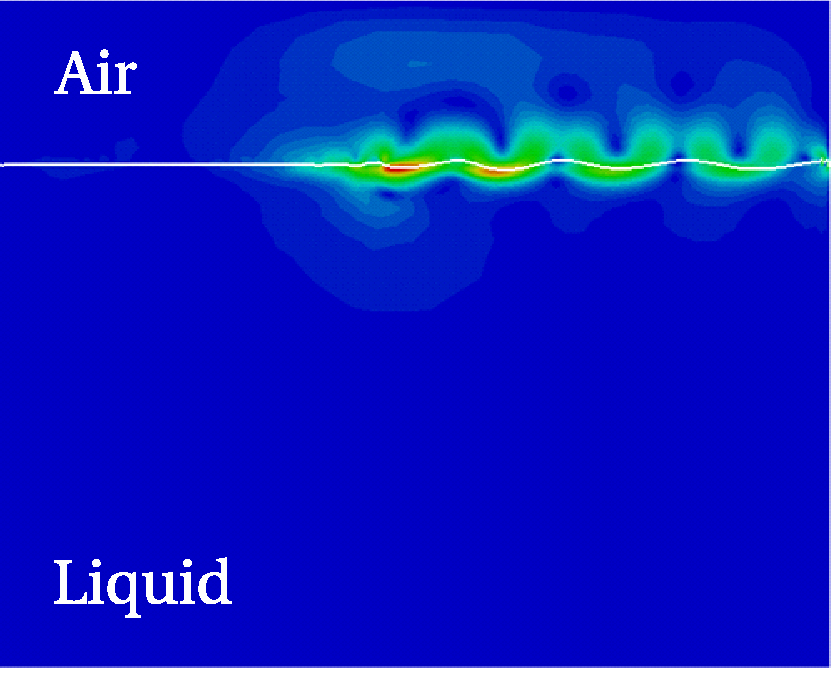
\includegraphics[width=\textwidth]{Chapter4/Graphics/UnstableInterface1.pdf}
	\caption{At a certain time increment (without mesh)}
    \label{fig:UnstableInterface1}
  \end{subfigure}
\qquad
 \begin{subfigure}[t]{0.4\textwidth}
    \centering
	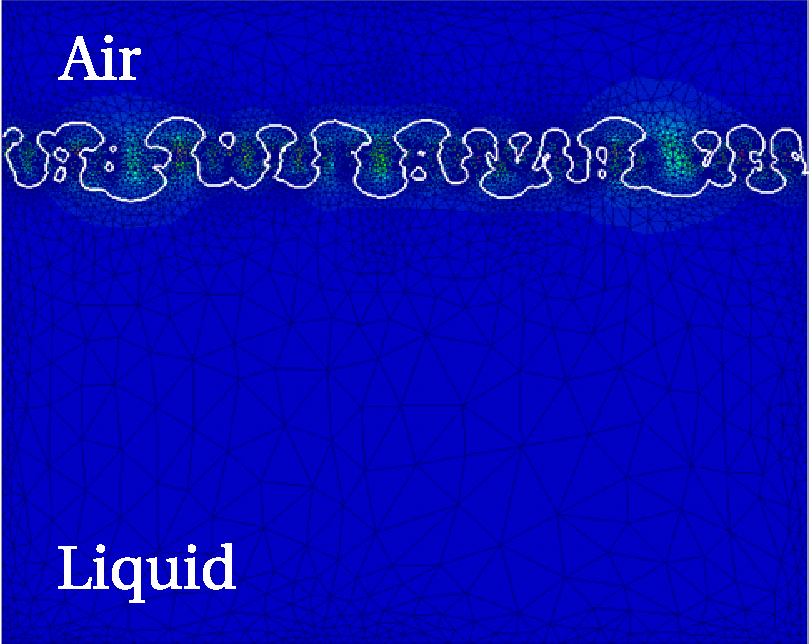
\includegraphics[width=\textwidth]{Chapter4/Graphics/UnstableInterface2.pdf}
	\caption{Another time increment (with mesh)}
    \label{fig:UnstableInterface2}
  \end{subfigure}
\caption{Interface destabilisation under the effect of high properties ratio across the interface.}
\end{figure}
%----------------------
%%---------
\subsubsection{Modified coupling}
In contrast to a classic coupling, here we attempt to modify the velocity field before feeding to the transport solver.
The main motivation for considering this approach is the lack of stability that we observed whenever the mechanical
properties of the fluids were different by several orders of magnitude.
The algorithm should simultaneously fulfil these requirements: 
\begin{itemize}
\itemsep0em
\item support high ratios of fluids density with close viscosities by preserving an non-oscillating interface,
\item maintain a horizontal level at the free surface of the melt,
\item follow shrinking metal surface profile in solidfying regions,
\item satisfy the mass conservation principle, essentially in the metal.
\end{itemize}
We want to process the original transport velocity by imposing a uniform motion (speed and direction) 
at the nodes of the free surface, and at the same time, be able to follow the pipe formation at the 
surface as a result of solidification shrinkage, as shown in \cref{fig:horizontal_liquid_surface}.
%----------------------
\begin{figureth}
% textwidth 
{0.8}
%path 
{Chapter4/Graphics/FreeSurface.pdf}
% caption
{Snapshot of a solidifying ingot by a cooling flux from the side. The profile of the actual surface changes in solid and mushy regions
to adapt the new density while staying perfectly horizontal in the liquid phase.}
% label
\label{fig:horizontal_liquid_surface}
\end{figureth}
%-----------------------------------
%
\comment{How to transport level set using velocity from momentum conservation DIRECTLY or AVERAGED PER ELEMENTS, 
show examples of instability/stability when using false/nominal air properties \\ 
Validation of LS transport: perform test case simulation of buoyancy driven air droplet in water by 2005Nagrath that I also have seen 
in Shyamprasad's masters report). => I didnt notice: what time step $\delta t$ did they use ? }
%
%----------------------
\begin{figureth}
% textwidth 
{0.8}
%path 
{Chapter4/Graphics/AvgTransport/BottomSideCooling.pdf}
% caption
{Treatment of liquid free surface in a) bottom and b) side heat extraction configurations. The dashed line represents the 
initial level of the free liquid surface.}
% label
\label{fig:bottom_side_cooling}
\end{figureth}
%-----------------------------------
The general idea is read the velocity around the interface up to a certain thickness, which may be the same 
thickness as the diffuse interface defined in \cref{sec:heaviside}, then compute a volumetric average
from all the elements in the thickness. This average is then given to the transport solver, which will apply
the same magnitude and direction to transport the interface. However, as we only need the transport velocity
to be uniform within the "100\% liquid" elements, it should not be the case for the other elements that belong 
either to the mushy zone or the solid region, where shrinkage is taking place.
Therefore, depending on the heat extraction configuration, two scenarios are possible. If heat extraction is far from
the interface, i.e. there is not direct contact as in \cref{fig:bottom_side_cooling}a, the surface area remains unchanged at any time, hence all the elements
around the interface are "100\% liquid". This happens when a bottom cooling is applied to the ingot. In contrast, if a side cooling 
is applied as shown in \cref{fig:bottom_side_cooling}b, the surface area of the interface will be reduced over time
as a consequence of the solid front progression. In this case, the average transport velocity should be computed only
from the elements belonging to the free surface. The remaining part of the interface which belongs to partial or full 
solid regions, is transported with Navier-Stokes output, which should be some orders of magnitude less than the velocity
imposed at the free surface, as a result of a decreasing permeability.

%
%--------------------------------
\section{Shrinkage without macrosegregation}
Explain how the flow and heat transfer in the air are not important \\ 
Give the strong form equations to be solved OR simply refer the previous section where the model was defined \\
Initial and boundary conditions for energy and momentum:  Initially we have liquid and air at rest. 
%--
\subsection{Al-7wt\% Si}
Present pseudo 1D case with results + discussion
%--
\subsection{Pb-3wt\% Sn}
Present 2D and 3D case with results + discussion
%--
%--------------------------------
\section{Shrinkage with macrosegregation}
Explain how the flow and heat transfer in the air are not important \\ 
Give the strong form equations to be solved OR simply refer the previous section where the model was defined \\
Initial and boundary conditions for energy and momentum:  Initially we have liquid and air at rest. 
%--
\subsection{Al-7wt\% Si}
Present pseudo 1D case with results + discussion
%--
\subsection{Pb-3wt\% Sn}
Present 2D and 3D case with results + discussion
%--

